\documentclass[border=5pt]{standalone}
\usepackage[T1]{fontenc}\usepackage{lmodern}\usepackage{pgfplots}
\pgfplotsset{compat=1.18}\begin{document}\sffamily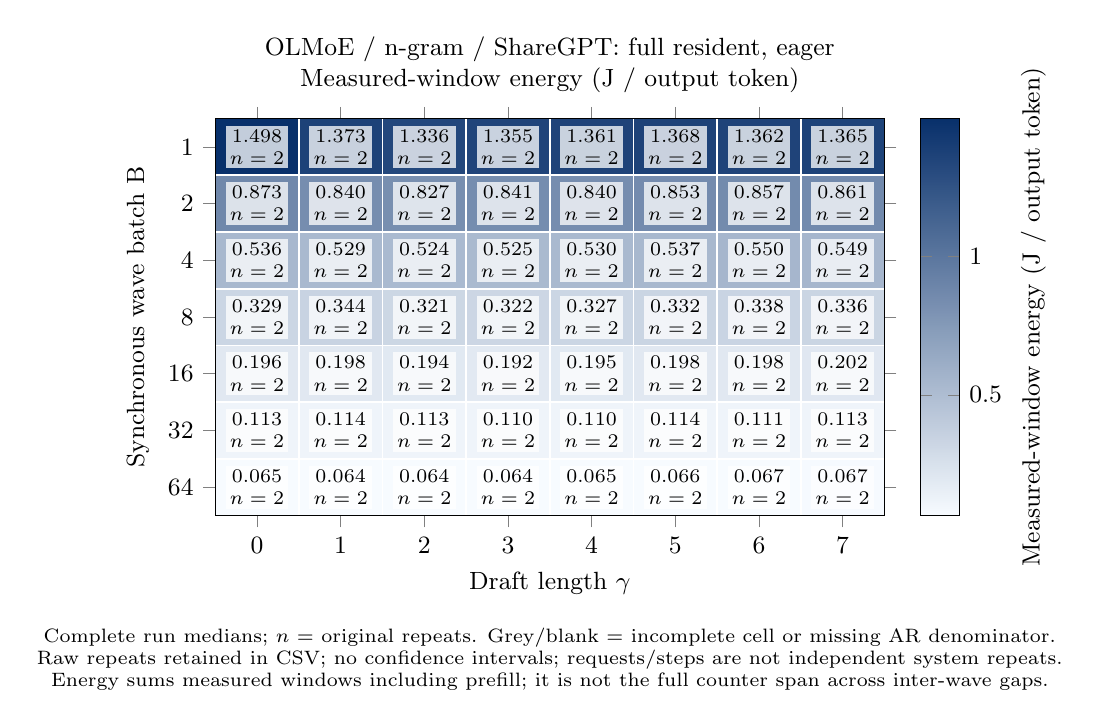
\begin{tikzpicture}
\begin{axis}[name=matrix,width=8.50cm,height=5.04cm,scale only axis,xmin=-.5,xmax=7.5,ymin=-.5,ymax=6.5,y dir=reverse,axis on top,tick align=outside,xtick={0,1,2,3,4,5,6,7},xticklabels={0,1,2,3,4,5,6,7},ytick={0,1,2,3,4,5,6},yticklabels={1,2,4,8,16,32,64},xlabel={Draft length $\gamma$},ylabel={Synchronous wave batch B},title={OLMoE / n-gram / ShareGPT: full resident, eager\\Measured-window energy (J / output token)},title style={align=center,font=\small},tick label style={font=\small},label style={font=\small},point meta min=0.0638260498047,point meta max=1.49822351074,colormap={matrixcolors}{rgb255=(247,251,255); rgb255=(245,249,254); rgb255=(242,247,252); rgb255=(240,245,251); rgb255=(237,243,249); rgb255=(235,241,248); rgb255=(233,239,246); rgb255=(230,237,245); rgb255=(228,235,243); rgb255=(225,233,242); rgb255=(223,231,240); rgb255=(221,229,239); rgb255=(218,227,237); rgb255=(216,225,236); rgb255=(214,223,234); rgb255=(211,221,233); rgb255=(209,219,231); rgb255=(206,216,230); rgb255=(204,214,228); rgb255=(202,212,227); rgb255=(199,210,225); rgb255=(197,208,224); rgb255=(194,206,222); rgb255=(192,204,221); rgb255=(190,202,219); rgb255=(187,200,218); rgb255=(185,198,217); rgb255=(182,196,215); rgb255=(180,194,214); rgb255=(178,192,212); rgb255=(175,190,211); rgb255=(173,188,209); rgb255=(171,186,208); rgb255=(168,184,206); rgb255=(166,182,205); rgb255=(163,180,203); rgb255=(161,178,202); rgb255=(159,176,200); rgb255=(156,174,199); rgb255=(154,172,197); rgb255=(151,170,196); rgb255=(149,168,194); rgb255=(147,166,193); rgb255=(144,164,191); rgb255=(142,162,190); rgb255=(139,160,188); rgb255=(137,158,187); rgb255=(135,156,185); rgb255=(132,154,184); rgb255=(130,152,182); rgb255=(128,150,181); rgb255=(125,147,180); rgb255=(123,145,178); rgb255=(120,143,177); rgb255=(118,141,175); rgb255=(116,139,174); rgb255=(113,137,172); rgb255=(111,135,171); rgb255=(108,133,169); rgb255=(106,131,168); rgb255=(104,129,166); rgb255=(101,127,165); rgb255=(99,125,163); rgb255=(96,123,162); rgb255=(94,121,160); rgb255=(92,119,159); rgb255=(89,117,157); rgb255=(87,115,156); rgb255=(84,113,154); rgb255=(82,111,153); rgb255=(80,109,151); rgb255=(77,107,150); rgb255=(75,105,148); rgb255=(73,103,147); rgb255=(70,101,145); rgb255=(68,99,144); rgb255=(65,97,143); rgb255=(63,95,141); rgb255=(61,93,140); rgb255=(58,91,138); rgb255=(56,89,137); rgb255=(53,87,135); rgb255=(51,85,134); rgb255=(49,83,132); rgb255=(46,80,131); rgb255=(44,78,129); rgb255=(41,76,128); rgb255=(39,74,126); rgb255=(37,72,125); rgb255=(34,70,123); rgb255=(32,68,122); rgb255=(30,66,120); rgb255=(27,64,119); rgb255=(25,62,117); rgb255=(22,60,116); rgb255=(20,58,114); rgb255=(18,56,113); rgb255=(15,54,111); rgb255=(13,52,110); rgb255=(10,50,108); rgb255=(8,48,107)},colorbar,colorbar style={ylabel={Measured-window energy (J / output token)},label style={font=\small},tick label style={font=\small}}]
\path[fill={rgb,255:red,8;green,48;blue,107},draw=white,line width=.6pt] (axis cs:-0.5,-0.5) rectangle (axis cs:0.5,0.5);
\node[align=center,font=\scriptsize,fill=white,fill opacity=.76,text opacity=1,inner sep=1.5pt] at (axis cs:0,0) {1.498\\$n=2$};
\path[fill={rgb,255:red,29;green,66;blue,120},draw=white,line width=.6pt] (axis cs:0.5,-0.5) rectangle (axis cs:1.5,0.5);
\node[align=center,font=\scriptsize,fill=white,fill opacity=.76,text opacity=1,inner sep=1.5pt] at (axis cs:1,0) {1.373\\$n=2$};
\path[fill={rgb,255:red,35;green,71;blue,124},draw=white,line width=.6pt] (axis cs:1.5,-0.5) rectangle (axis cs:2.5,0.5);
\node[align=center,font=\scriptsize,fill=white,fill opacity=.76,text opacity=1,inner sep=1.5pt] at (axis cs:2,0) {1.336\\$n=2$};
\path[fill={rgb,255:red,32;green,68;blue,122},draw=white,line width=.6pt] (axis cs:2.5,-0.5) rectangle (axis cs:3.5,0.5);
\node[align=center,font=\scriptsize,fill=white,fill opacity=.76,text opacity=1,inner sep=1.5pt] at (axis cs:3,0) {1.355\\$n=2$};
\path[fill={rgb,255:red,31;green,67;blue,121},draw=white,line width=.6pt] (axis cs:3.5,-0.5) rectangle (axis cs:4.5,0.5);
\node[align=center,font=\scriptsize,fill=white,fill opacity=.76,text opacity=1,inner sep=1.5pt] at (axis cs:4,0) {1.361\\$n=2$};
\path[fill={rgb,255:red,30;green,66;blue,120},draw=white,line width=.6pt] (axis cs:4.5,-0.5) rectangle (axis cs:5.5,0.5);
\node[align=center,font=\scriptsize,fill=white,fill opacity=.76,text opacity=1,inner sep=1.5pt] at (axis cs:5,0) {1.368\\$n=2$};
\path[fill={rgb,255:red,31;green,67;blue,121},draw=white,line width=.6pt] (axis cs:5.5,-0.5) rectangle (axis cs:6.5,0.5);
\node[align=center,font=\scriptsize,fill=white,fill opacity=.76,text opacity=1,inner sep=1.5pt] at (axis cs:6,0) {1.362\\$n=2$};
\path[fill={rgb,255:red,30;green,67;blue,121},draw=white,line width=.6pt] (axis cs:6.5,-0.5) rectangle (axis cs:7.5,0.5);
\node[align=center,font=\scriptsize,fill=white,fill opacity=.76,text opacity=1,inner sep=1.5pt] at (axis cs:7,0) {1.365\\$n=2$};
\path[fill={rgb,255:red,112;green,136;blue,171},draw=white,line width=.6pt] (axis cs:-0.5,0.5) rectangle (axis cs:0.5,1.5);
\node[align=center,font=\scriptsize,fill=white,fill opacity=.76,text opacity=1,inner sep=1.5pt] at (axis cs:0,1) {0.873\\$n=2$};
\path[fill={rgb,255:red,118;green,141;blue,175},draw=white,line width=.6pt] (axis cs:0.5,0.5) rectangle (axis cs:1.5,1.5);
\node[align=center,font=\scriptsize,fill=white,fill opacity=.76,text opacity=1,inner sep=1.5pt] at (axis cs:1,1) {0.840\\$n=2$};
\path[fill={rgb,255:red,120;green,143;blue,176},draw=white,line width=.6pt] (axis cs:1.5,0.5) rectangle (axis cs:2.5,1.5);
\node[align=center,font=\scriptsize,fill=white,fill opacity=.76,text opacity=1,inner sep=1.5pt] at (axis cs:2,1) {0.827\\$n=2$};
\path[fill={rgb,255:red,117;green,141;blue,175},draw=white,line width=.6pt] (axis cs:2.5,0.5) rectangle (axis cs:3.5,1.5);
\node[align=center,font=\scriptsize,fill=white,fill opacity=.76,text opacity=1,inner sep=1.5pt] at (axis cs:3,1) {0.841\\$n=2$};
\path[fill={rgb,255:red,118;green,141;blue,175},draw=white,line width=.6pt] (axis cs:3.5,0.5) rectangle (axis cs:4.5,1.5);
\node[align=center,font=\scriptsize,fill=white,fill opacity=.76,text opacity=1,inner sep=1.5pt] at (axis cs:4,1) {0.840\\$n=2$};
\path[fill={rgb,255:red,116;green,139;blue,174},draw=white,line width=.6pt] (axis cs:4.5,0.5) rectangle (axis cs:5.5,1.5);
\node[align=center,font=\scriptsize,fill=white,fill opacity=.76,text opacity=1,inner sep=1.5pt] at (axis cs:5,1) {0.853\\$n=2$};
\path[fill={rgb,255:red,115;green,139;blue,173},draw=white,line width=.6pt] (axis cs:5.5,0.5) rectangle (axis cs:6.5,1.5);
\node[align=center,font=\scriptsize,fill=white,fill opacity=.76,text opacity=1,inner sep=1.5pt] at (axis cs:6,1) {0.857\\$n=2$};
\path[fill={rgb,255:red,114;green,138;blue,173},draw=white,line width=.6pt] (axis cs:6.5,0.5) rectangle (axis cs:7.5,1.5);
\node[align=center,font=\scriptsize,fill=white,fill opacity=.76,text opacity=1,inner sep=1.5pt] at (axis cs:7,1) {0.861\\$n=2$};
\path[fill={rgb,255:red,168;green,184;blue,206},draw=white,line width=.6pt] (axis cs:-0.5,1.5) rectangle (axis cs:0.5,2.5);
\node[align=center,font=\scriptsize,fill=white,fill opacity=.76,text opacity=1,inner sep=1.5pt] at (axis cs:0,2) {0.536\\$n=2$};
\path[fill={rgb,255:red,169;green,185;blue,207},draw=white,line width=.6pt] (axis cs:0.5,1.5) rectangle (axis cs:1.5,2.5);
\node[align=center,font=\scriptsize,fill=white,fill opacity=.76,text opacity=1,inner sep=1.5pt] at (axis cs:1,2) {0.529\\$n=2$};
\path[fill={rgb,255:red,170;green,186;blue,208},draw=white,line width=.6pt] (axis cs:1.5,1.5) rectangle (axis cs:2.5,2.5);
\node[align=center,font=\scriptsize,fill=white,fill opacity=.76,text opacity=1,inner sep=1.5pt] at (axis cs:2,2) {0.524\\$n=2$};
\path[fill={rgb,255:red,170;green,186;blue,207},draw=white,line width=.6pt] (axis cs:2.5,1.5) rectangle (axis cs:3.5,2.5);
\node[align=center,font=\scriptsize,fill=white,fill opacity=.76,text opacity=1,inner sep=1.5pt] at (axis cs:3,2) {0.525\\$n=2$};
\path[fill={rgb,255:red,169;green,185;blue,207},draw=white,line width=.6pt] (axis cs:3.5,1.5) rectangle (axis cs:4.5,2.5);
\node[align=center,font=\scriptsize,fill=white,fill opacity=.76,text opacity=1,inner sep=1.5pt] at (axis cs:4,2) {0.530\\$n=2$};
\path[fill={rgb,255:red,168;green,184;blue,206},draw=white,line width=.6pt] (axis cs:4.5,1.5) rectangle (axis cs:5.5,2.5);
\node[align=center,font=\scriptsize,fill=white,fill opacity=.76,text opacity=1,inner sep=1.5pt] at (axis cs:5,2) {0.537\\$n=2$};
\path[fill={rgb,255:red,166;green,182;blue,205},draw=white,line width=.6pt] (axis cs:5.5,1.5) rectangle (axis cs:6.5,2.5);
\node[align=center,font=\scriptsize,fill=white,fill opacity=.76,text opacity=1,inner sep=1.5pt] at (axis cs:6,2) {0.550\\$n=2$};
\path[fill={rgb,255:red,166;green,182;blue,205},draw=white,line width=.6pt] (axis cs:6.5,1.5) rectangle (axis cs:7.5,2.5);
\node[align=center,font=\scriptsize,fill=white,fill opacity=.76,text opacity=1,inner sep=1.5pt] at (axis cs:7,2) {0.549\\$n=2$};
\path[fill={rgb,255:red,203;green,214;blue,228},draw=white,line width=.6pt] (axis cs:-0.5,2.5) rectangle (axis cs:0.5,3.5);
\node[align=center,font=\scriptsize,fill=white,fill opacity=.76,text opacity=1,inner sep=1.5pt] at (axis cs:0,3) {0.329\\$n=2$};
\path[fill={rgb,255:red,200;green,211;blue,226},draw=white,line width=.6pt] (axis cs:0.5,2.5) rectangle (axis cs:1.5,3.5);
\node[align=center,font=\scriptsize,fill=white,fill opacity=.76,text opacity=1,inner sep=1.5pt] at (axis cs:1,3) {0.344\\$n=2$};
\path[fill={rgb,255:red,204;green,215;blue,228},draw=white,line width=.6pt] (axis cs:1.5,2.5) rectangle (axis cs:2.5,3.5);
\node[align=center,font=\scriptsize,fill=white,fill opacity=.76,text opacity=1,inner sep=1.5pt] at (axis cs:2,3) {0.321\\$n=2$};
\path[fill={rgb,255:red,204;green,214;blue,228},draw=white,line width=.6pt] (axis cs:2.5,2.5) rectangle (axis cs:3.5,3.5);
\node[align=center,font=\scriptsize,fill=white,fill opacity=.76,text opacity=1,inner sep=1.5pt] at (axis cs:3,3) {0.322\\$n=2$};
\path[fill={rgb,255:red,203;green,214;blue,228},draw=white,line width=.6pt] (axis cs:3.5,2.5) rectangle (axis cs:4.5,3.5);
\node[align=center,font=\scriptsize,fill=white,fill opacity=.76,text opacity=1,inner sep=1.5pt] at (axis cs:4,3) {0.327\\$n=2$};
\path[fill={rgb,255:red,202;green,213;blue,227},draw=white,line width=.6pt] (axis cs:4.5,2.5) rectangle (axis cs:5.5,3.5);
\node[align=center,font=\scriptsize,fill=white,fill opacity=.76,text opacity=1,inner sep=1.5pt] at (axis cs:5,3) {0.332\\$n=2$};
\path[fill={rgb,255:red,201;green,212;blue,227},draw=white,line width=.6pt] (axis cs:5.5,2.5) rectangle (axis cs:6.5,3.5);
\node[align=center,font=\scriptsize,fill=white,fill opacity=.76,text opacity=1,inner sep=1.5pt] at (axis cs:6,3) {0.338\\$n=2$};
\path[fill={rgb,255:red,202;green,213;blue,227},draw=white,line width=.6pt] (axis cs:6.5,2.5) rectangle (axis cs:7.5,3.5);
\node[align=center,font=\scriptsize,fill=white,fill opacity=.76,text opacity=1,inner sep=1.5pt] at (axis cs:7,3) {0.336\\$n=2$};
\path[fill={rgb,255:red,225;green,232;blue,241},draw=white,line width=.6pt] (axis cs:-0.5,3.5) rectangle (axis cs:0.5,4.5);
\node[align=center,font=\scriptsize,fill=white,fill opacity=.76,text opacity=1,inner sep=1.5pt] at (axis cs:0,4) {0.196\\$n=2$};
\path[fill={rgb,255:red,225;green,232;blue,241},draw=white,line width=.6pt] (axis cs:0.5,3.5) rectangle (axis cs:1.5,4.5);
\node[align=center,font=\scriptsize,fill=white,fill opacity=.76,text opacity=1,inner sep=1.5pt] at (axis cs:1,4) {0.198\\$n=2$};
\path[fill={rgb,255:red,225;green,233;blue,242},draw=white,line width=.6pt] (axis cs:1.5,3.5) rectangle (axis cs:2.5,4.5);
\node[align=center,font=\scriptsize,fill=white,fill opacity=.76,text opacity=1,inner sep=1.5pt] at (axis cs:2,4) {0.194\\$n=2$};
\path[fill={rgb,255:red,226;green,233;blue,242},draw=white,line width=.6pt] (axis cs:2.5,3.5) rectangle (axis cs:3.5,4.5);
\node[align=center,font=\scriptsize,fill=white,fill opacity=.76,text opacity=1,inner sep=1.5pt] at (axis cs:3,4) {0.192\\$n=2$};
\path[fill={rgb,255:red,225;green,233;blue,242},draw=white,line width=.6pt] (axis cs:3.5,3.5) rectangle (axis cs:4.5,4.5);
\node[align=center,font=\scriptsize,fill=white,fill opacity=.76,text opacity=1,inner sep=1.5pt] at (axis cs:4,4) {0.195\\$n=2$};
\path[fill={rgb,255:red,225;green,232;blue,241},draw=white,line width=.6pt] (axis cs:4.5,3.5) rectangle (axis cs:5.5,4.5);
\node[align=center,font=\scriptsize,fill=white,fill opacity=.76,text opacity=1,inner sep=1.5pt] at (axis cs:5,4) {0.198\\$n=2$};
\path[fill={rgb,255:red,225;green,232;blue,241},draw=white,line width=.6pt] (axis cs:5.5,3.5) rectangle (axis cs:6.5,4.5);
\node[align=center,font=\scriptsize,fill=white,fill opacity=.76,text opacity=1,inner sep=1.5pt] at (axis cs:6,4) {0.198\\$n=2$};
\path[fill={rgb,255:red,224;green,231;blue,241},draw=white,line width=.6pt] (axis cs:6.5,3.5) rectangle (axis cs:7.5,4.5);
\node[align=center,font=\scriptsize,fill=white,fill opacity=.76,text opacity=1,inner sep=1.5pt] at (axis cs:7,4) {0.202\\$n=2$};
\path[fill={rgb,255:red,239;green,244;blue,250},draw=white,line width=.6pt] (axis cs:-0.5,4.5) rectangle (axis cs:0.5,5.5);
\node[align=center,font=\scriptsize,fill=white,fill opacity=.76,text opacity=1,inner sep=1.5pt] at (axis cs:0,5) {0.113\\$n=2$};
\path[fill={rgb,255:red,239;green,244;blue,250},draw=white,line width=.6pt] (axis cs:0.5,4.5) rectangle (axis cs:1.5,5.5);
\node[align=center,font=\scriptsize,fill=white,fill opacity=.76,text opacity=1,inner sep=1.5pt] at (axis cs:1,5) {0.114\\$n=2$};
\path[fill={rgb,255:red,239;green,244;blue,250},draw=white,line width=.6pt] (axis cs:1.5,4.5) rectangle (axis cs:2.5,5.5);
\node[align=center,font=\scriptsize,fill=white,fill opacity=.76,text opacity=1,inner sep=1.5pt] at (axis cs:2,5) {0.113\\$n=2$};
\path[fill={rgb,255:red,239;green,244;blue,250},draw=white,line width=.6pt] (axis cs:2.5,4.5) rectangle (axis cs:3.5,5.5);
\node[align=center,font=\scriptsize,fill=white,fill opacity=.76,text opacity=1,inner sep=1.5pt] at (axis cs:3,5) {0.110\\$n=2$};
\path[fill={rgb,255:red,239;green,244;blue,250},draw=white,line width=.6pt] (axis cs:3.5,4.5) rectangle (axis cs:4.5,5.5);
\node[align=center,font=\scriptsize,fill=white,fill opacity=.76,text opacity=1,inner sep=1.5pt] at (axis cs:4,5) {0.110\\$n=2$};
\path[fill={rgb,255:red,239;green,244;blue,250},draw=white,line width=.6pt] (axis cs:4.5,4.5) rectangle (axis cs:5.5,5.5);
\node[align=center,font=\scriptsize,fill=white,fill opacity=.76,text opacity=1,inner sep=1.5pt] at (axis cs:5,5) {0.114\\$n=2$};
\path[fill={rgb,255:red,239;green,244;blue,250},draw=white,line width=.6pt] (axis cs:5.5,4.5) rectangle (axis cs:6.5,5.5);
\node[align=center,font=\scriptsize,fill=white,fill opacity=.76,text opacity=1,inner sep=1.5pt] at (axis cs:6,5) {0.111\\$n=2$};
\path[fill={rgb,255:red,239;green,244;blue,250},draw=white,line width=.6pt] (axis cs:6.5,4.5) rectangle (axis cs:7.5,5.5);
\node[align=center,font=\scriptsize,fill=white,fill opacity=.76,text opacity=1,inner sep=1.5pt] at (axis cs:7,5) {0.113\\$n=2$};
\path[fill={rgb,255:red,247;green,251;blue,255},draw=white,line width=.6pt] (axis cs:-0.5,5.5) rectangle (axis cs:0.5,6.5);
\node[align=center,font=\scriptsize,fill=white,fill opacity=.76,text opacity=1,inner sep=1.5pt] at (axis cs:0,6) {0.065\\$n=2$};
\path[fill={rgb,255:red,247;green,251;blue,255},draw=white,line width=.6pt] (axis cs:0.5,5.5) rectangle (axis cs:1.5,6.5);
\node[align=center,font=\scriptsize,fill=white,fill opacity=.76,text opacity=1,inner sep=1.5pt] at (axis cs:1,6) {0.064\\$n=2$};
\path[fill={rgb,255:red,247;green,251;blue,255},draw=white,line width=.6pt] (axis cs:1.5,5.5) rectangle (axis cs:2.5,6.5);
\node[align=center,font=\scriptsize,fill=white,fill opacity=.76,text opacity=1,inner sep=1.5pt] at (axis cs:2,6) {0.064\\$n=2$};
\path[fill={rgb,255:red,247;green,251;blue,255},draw=white,line width=.6pt] (axis cs:2.5,5.5) rectangle (axis cs:3.5,6.5);
\node[align=center,font=\scriptsize,fill=white,fill opacity=.76,text opacity=1,inner sep=1.5pt] at (axis cs:3,6) {0.064\\$n=2$};
\path[fill={rgb,255:red,247;green,251;blue,255},draw=white,line width=.6pt] (axis cs:3.5,5.5) rectangle (axis cs:4.5,6.5);
\node[align=center,font=\scriptsize,fill=white,fill opacity=.76,text opacity=1,inner sep=1.5pt] at (axis cs:4,6) {0.065\\$n=2$};
\path[fill={rgb,255:red,247;green,251;blue,255},draw=white,line width=.6pt] (axis cs:4.5,5.5) rectangle (axis cs:5.5,6.5);
\node[align=center,font=\scriptsize,fill=white,fill opacity=.76,text opacity=1,inner sep=1.5pt] at (axis cs:5,6) {0.066\\$n=2$};
\path[fill={rgb,255:red,247;green,251;blue,255},draw=white,line width=.6pt] (axis cs:5.5,5.5) rectangle (axis cs:6.5,6.5);
\node[align=center,font=\scriptsize,fill=white,fill opacity=.76,text opacity=1,inner sep=1.5pt] at (axis cs:6,6) {0.067\\$n=2$};
\path[fill={rgb,255:red,246;green,250;blue,255},draw=white,line width=.6pt] (axis cs:6.5,5.5) rectangle (axis cs:7.5,6.5);
\node[align=center,font=\scriptsize,fill=white,fill opacity=.76,text opacity=1,inner sep=1.5pt] at (axis cs:7,6) {0.067\\$n=2$};
\end{axis}
\node[below=1.3cm,align=center,font=\scriptsize] at (matrix.south) {Complete run medians; $n$ = original repeats. Grey/blank = incomplete cell or missing AR denominator.\\Raw repeats retained in CSV; no confidence intervals; requests/steps are not independent system repeats.\\Energy sums measured windows including prefill; it is not the full counter span across inter-wave gaps.};
\end{tikzpicture}\end{document}
